\documentclass{oblivoir}
\usepackage{amsmath,amssymb,amsthm,kotex,paralist,kswrapfig,graphicx}

\usepackage[skipabove=10pt,innertopmargin=10pt]{mdframed}

\usepackage{tabto,pifont}
\TabPositions{0.2\textwidth,0.4\textwidth,0.6\textwidth,0.8\textwidth}
\newcommand\tabb[5]{\par\bigskip\noindent\ding{172}\:{\ensuremath{#1}}
\tab\ding{173}\:\:{\ensuremath{#2}}\tab\ding{174}\:\:{\ensuremath{#3}}
\tab\ding{175}\:\:{\ensuremath{#4}}\tab\ding{176}\:\:{\ensuremath{#5}}}
\newcommand\tabfive[5]{\par\medskip\noindent\ding{172}\:\:{\ensuremath{#1}}\\
\ding{173}\:\:{\ensuremath{#2}}\\\ding{174}\:\:{\ensuremath{#3}}\\
\ding{175}\:\:{\ensuremath{#4}}\\\ding{176}\:\:{\ensuremath{#5}}}

\usepackage{enumitem}
\setlist[enumerate]{label=(\arabic*)}

\newcounter{num}
\newcommand{\defi}[1]
{\noindent\refstepcounter{num}\textbf{정의 \arabic{num}) #1}\par\noindent}
\newcommand{\theo}[1]
{\noindent\refstepcounter{num}\textbf{정리 \arabic{num}) #1}\par\noindent}
\newcommand{\exam}[1]
{\bigskip\bigskip\noindent\refstepcounter{num}\textbf{예시 \arabic{num}) #1}\par\noindent}
\newcommand{\prob}[1]
{\bigskip\bigskip\noindent\refstepcounter{num}\textbf{문제 \arabic{num}) #1}\par\noindent}
\newcommand{\proo}
{\bigskip\textsf{증명)}\par}

\newcommand{\ans}{
{\par
\raggedleft\textbf{답 : (\qquad\qquad\qquad\qquad\qquad\qquad)}
\par}\bigskip\bigskip}
\newcommand{\procedure}[1]{\begin{mdframed}\vspace{#1\textheight}\end{mdframed}}
\newcommand\an[1]{\par\bigskip\noindent\textbf{문제 #1)}\\}

\newcommand{\pb}[1]%\Phantom + fBox
{\fbox{\phantom{\ensuremath{#1}}}}
\newcommand\ba{\,|\,}

\let\oldsection\section
\renewcommand\section{\clearpage\oldsection}

\renewcommand{\arraystretch}{1.5}

\let\emph\textsf
%%%%
\begin{document}

\title{윤영 : 10 함수(1)}
\author{}
\date{\today}
\maketitle
\tableofcontents
\newpage

%%
\section{함수}
%
\exam{}\label{nation1}
두 집합 
\begin{align*}
나라&=\{대한민국, 일본, 미국\}\\
도시&=\{서울, 시카고, 워싱턴, 도쿄, 춘천, 부산\}
\end{align*}
을 나란히 놓고, 각각의 나라에 그 나라의 수도를 연결하자.
\begin{figure*}[h!]
\centering
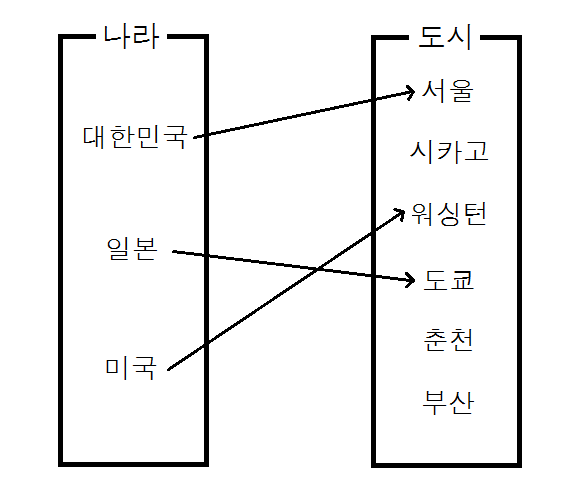
\includegraphics[width=0.4\textwidth]{nation-capital}
\end{figure*}

\begin{mdframed}[skipbelow=10pt]
%
\defi{대응과 함수, 정의역, 공역}
\begin{enumerate}
\item
이처럼 두 집합 \(X\), \(Y\)에 대하여 집합 \(X\)의 원소에 집합 \(Y\)의 원소를 짝지어주는 것을 집합 \(X\)에서 집합 \(Y\)로의 \emph{대응}이라고 한다.
\item
특히, 집합 \(X\)의 각 원소에 집합 \(Y\)의 원소가 하나씩 대응될 때, 이 대응 \(f\)를 집합 \(X\)에서 집합 \(Y\)로의 \emph{함수}라고 하고 이것을 기호로
\[f:X\to Y\]
와 같이 나타낸다.
이때 집합 \(X\)를 함수 \(f\)의 \emph{정의역}, 집합 \(Y\)를 함수 \(f\)의 \emph{공역}이라고 부른다.
\end{enumerate}
\end{mdframed}
따라서, 위의 예제 \ref{nation1}\는 대응이면서 함수이다.
이 함수의 정의역은 `나라'이고, 공역은 `도시'이다.

\begin{mdframed}[skipbelow=10pt]
%
\defi{함숫값, 치역}
함수 \(f\)에 의하여 정의역 \(X\)의 원소 \(x\)가 공역 \(Y\)의 원소 \(y\)에 대응될 때, 이것을 기호로
\[y=f(x)\]
와 같이 나타내고, \(f(x)\)를 함수 \(f\)에 의한 \(x\)의 \emph{함숫값}이라고 한다.
또 함숫값 전체의 집합 \(\{f(x)\ba x\in X\}\)\를 함수 \(f\)의 \emph{치역}이라고 한다.
이때 치역은 공역의 부분집합이다.% 사이에는 다음 관계가 성립한다.
%\[치역\subset 공역\]
\end{mdframed}
따라서, 위의 예시 \ref{nation1}의 함수에서 \(f(대한민국)=서울\), \(f(일본)=도쿄\), \(f(미국)=워싱턴\)이고, 치역은
\begin{align*}
치역
&=\{f(x)\ba x\in나라\}=\{f(대한민국),f(일본),f(미국)\}\\
&=\{서울,도쿄,워싱턴\}
\end{align*}

\vspace{-10pt}
%
\exam{}\label{nation2}
아래의 세 그림은
(1) 나라와 도시를 연결,
(2) 수도와 나라를 연결,
(3) 도시와 나라를 연결한 것이다.

\begin{figure*}[h!]
\centering
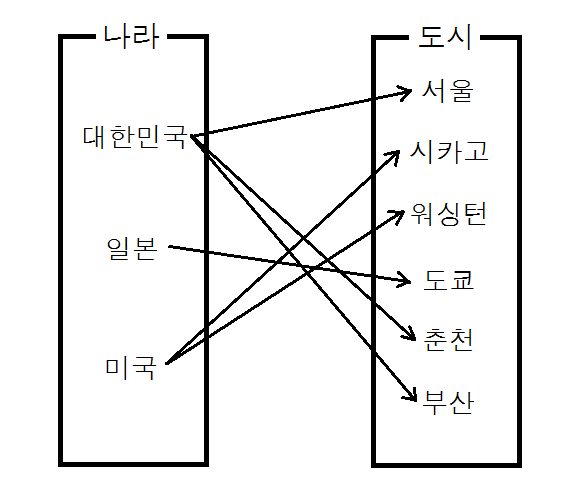
\includegraphics[width=0.3\textwidth]{nation-city}
~
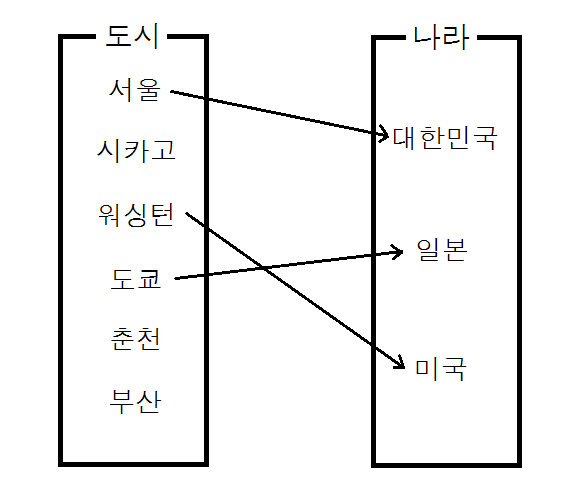
\includegraphics[width=0.3\textwidth]{capital-nation}
~
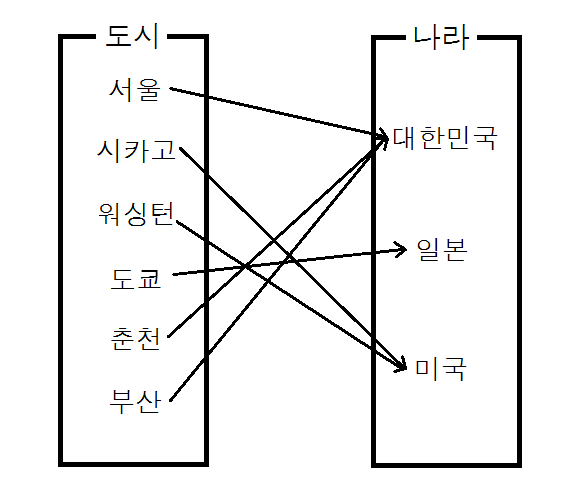
\includegraphics[width=0.3\textwidth]{city-nation}
\end{figure*}

\begin{enumerate}
\item
함수는 \(X\)의 각 원소가 \(Y\)의 원소에 \emph{하나씩} 대응되어야 하는데 \(X\)의 원소인 대한민국은  \(Y\)의 세 개 원소 서울, 춘천, 부산에 대응되었다.
따라서 함수가 아니다.
\item
함수는 \(X\)의 \emph{각 원소}가 \(Y\)의 원소에 하나씩 대응되어야 하는데 \(X\)의 원소인 시카고는  \(Y\)의 원소에 대응되지 않았다.
따라서 함수가 아니다.
\item
이 대응은 함수의 조건을 모두 만족시키므로 함수이다.
이때 정의역은 `도시', 공역은 `나라'이며 치역은 \(\{대한민국, 일본, 미국\}\)으로 공역과 같다.
\end{enumerate}

%
\prob{}
다음 대응 중 함수인 것을 찾고, 함수인 경우 정의역, 공역, 치역을 각각 말하여라.

\begin{figure*}[h!]
\centering
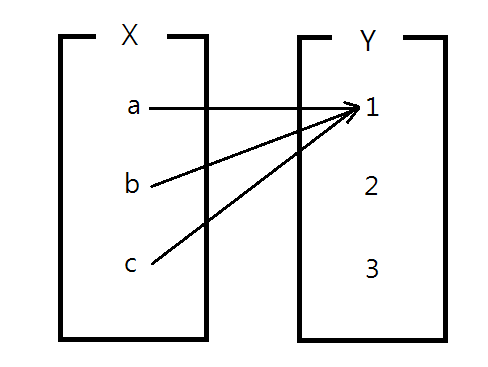
\includegraphics[width=0.3\textwidth]{function_1}
~
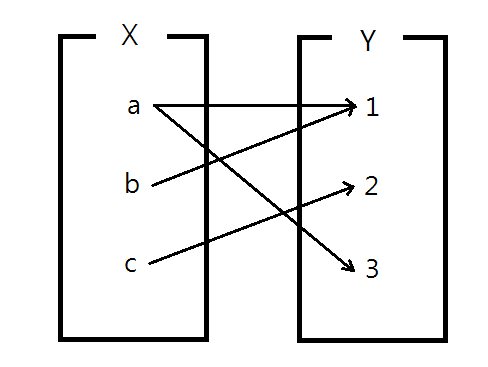
\includegraphics[width=0.3\textwidth]{function_2}
~
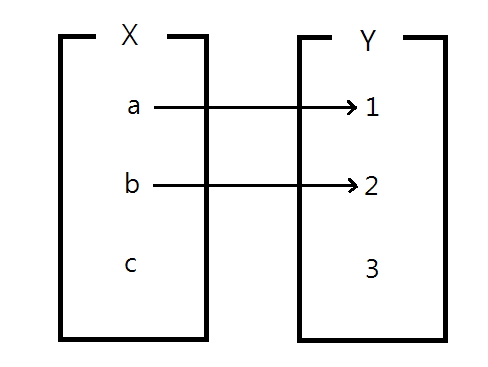
\includegraphics[width=0.3\textwidth]{function_3}
\par\noindent
(1)
\qquad\qquad\qquad\qquad\quad\:\:
(2)
\qquad\qquad\qquad\qquad\quad\:\:
(3)
\end{figure*}

%\begin{enumerate}
%\item
%함수이다 / 함수가 아니다,\\
%\(정의역=\{\phantom{1,2,3,}\}\),
%\(공역=\{\phantom{1,2,3,}\}\),
%\(치역=\{\phantom{1,2,3,}\}\)
%\item
%함수이다 / 함수가 아니다,\\
%\(정의역=\{\phantom{1,2,3,}\}\),
%\(공역=\{\phantom{1,2,3,}\}\),
%\(치역=\{\phantom{1,2,3,}\}\)
%\item
%함수이다 / 함수가 아니다,\\
%\(정의역=\{\phantom{1,2,3,}\}\),
%\(공역=\{\phantom{1,2,3,}\}\),
%\(치역=\{\phantom{1,2,3,}\}\)
%\end{enumerate}
\vspace{0.1\textheight}

함수 \(y=f(x)\)의 정의역이나 공역이 주어지지 않은 경우에는 함숫값 \(f(x)\)가 정의되는 \(x\)의 값 전체의 집합을 정의역으로 하고, 실수 전체의 집합을 공역으로 한다.

%
\exam{}
%\begin{enumerate}
%\item
함수 \(y=-x+3\)에서 모든 실수 \(x\)에 대하여 \(y\)의 값이 \(-x+3\)으로 한 개씩 정해지므로 함수 \(y=-x+3\)의 정의역과 치역은 모두 실수 전체의 집합이다.
%또한 모든 실수 \(y\)값이 함숫값이 될 수 있으므로 치역도 실수 전체의 집합이다.
%\item
%함수 \(y=\frac1{x^2-4}\)에서 \(x=2\)이거나 \(x=-2\)가 되면 \(y\)의 값이 정해질 수 없다.
%따라서 정의역은 \(\{x\ba x\neq\pm2\}\)이고 공역은 실수 전체의 집합이다.
%\end{enumerate}

%
\prob{}\label{domain_range}
다음 함수의 정의역과 치역을 말하여라.
\begin{enumerate}
\item
\(y=2x-3\)
\item
\(y=x^2-3\)
\item
\(y=\frac1x\)
\item
\(y=4\)
\end{enumerate}
{\par\raggedleft\textbf{답 :
(1)\:\:정의역=\phantom{실수 전체 집합}, 치역=\phantom{실수 전체 집합}}\par}
{\par\raggedleft\textbf{
(2)\:\:정의역=\phantom{실수 전체 집합}, 치역=\phantom{실수 전체 집합}}\par}
{\par\raggedleft\textbf{
(3)\:\:정의역=\phantom{실수 전체 집합}, 치역=\phantom{실수 전체 집합}}\par}
{\par\raggedleft\textbf{
(4)\:\:정의역=\phantom{실수 전체 집합}, 치역=\phantom{실수 전체 집합}}\par}
\bigskip

\begin{mdframed}
%
\defi{}
두 함수 \(f:X\to Y\), \(g:X\to Y\)에서 정의역의 모든 원소 \(x\)에 대하여 \(f(x)=g(x)\)일 때, 두 함수 \(f\)와 \(g\)는 서로 같다고 하며, 이것을 기호로
\[f=g\]
와 같이 나타낸다.
\end{mdframed}

%
\exam{}
\begin{enumerate}
\item
\(X=\{0,1\}\)을 정의역으로 하는 두 함수 \(f(x)=x\)와 \(g(x)=x^2\)\은 \\
\(f(0)=0=g(0)\), \(f(1)=1=g(1)\)이므로 \(f=g\)이다.
\item
\(X=\{1,2,3\}\)을 정의역으로 하는 두 함수 \(f(x)=x^2-x\)와 \(g(x)=2x-2\)\은
 \(f(1)=0=g(1)\), \(f(2)=2=g(2)\)이지만 \(f(3)=6\neq4=g(3)\)이므로 \(f\neq g\)이다.
\end{enumerate}

%
\prob{}
\begin{enumerate}
\item
\(X=\{-1,0,1\}\)을 정의역으로 하는 두 함수 \(f(x)=|x|\)와 \(g(x)=x^2\)\은\\
서로 (같다 / 다르다).
\item
\(X=\{-1,1\}\)을 정의역으로 하는 두 함수 \(f(x)=x+1\)와 \(g(x)=x-1\)\은\\
서로 (같다 / 다르다).
\end{enumerate}

%%
\section{함수의 그래프}

\begin{mdframed}
%
\defi{함수의 그래프}
함수 \(f:X\to Y\)에 대하여 정의역 \(X\)의 원소 \(x\)와 이에 대응하는 함숫값 \(f(x)\)의 순서쌍 전체의 집합인
\[\{(x,f(x))\ba x\in X\}\]
를 함수 \(f\)의 \emph{그래프}라고 한다.
\end{mdframed}

\kswrapfig[Pos=r]{first_graph}{
%
\exam{}
예를 들어 정의역이 \(X=\{1,2,3\}\)인 함수 \(f(x)=x+1\)의 그래프는 \(f(1)=2\), \(f(2)=3\), \(f(3)=4\)이므로
\[\{(1,2),(2,3),(3,4)\}\]
이다.

이것을 좌표평면 위에 나타내면 오른쪽 그림과 같다.
}

\kswrapfig[Pos=r]{second_graph}{
%
\exam{}
예시 \ref{domain_range} (1)의 함수 \(y=2x-3\)는 정의역이 실수 전체이다.
따라서 그래프인 \(\{(x,2x-3)\ba x\text{는 실수}\}\)는 무한집합이고
\[(0,-3), (1,-1), (2,1), (3,3)\]
등의 점을 원소로 포함한다.
이 무한개의 점들을 좌표평면에 찍으면 오른쪽 그림과 같은 직선이 나온다.
}

\clearpage
%
\prob{}
다음 그림 중 함수의 그래프인 것을 모두 찾아라.
\begin{figure}[h!]
\centering\noindent
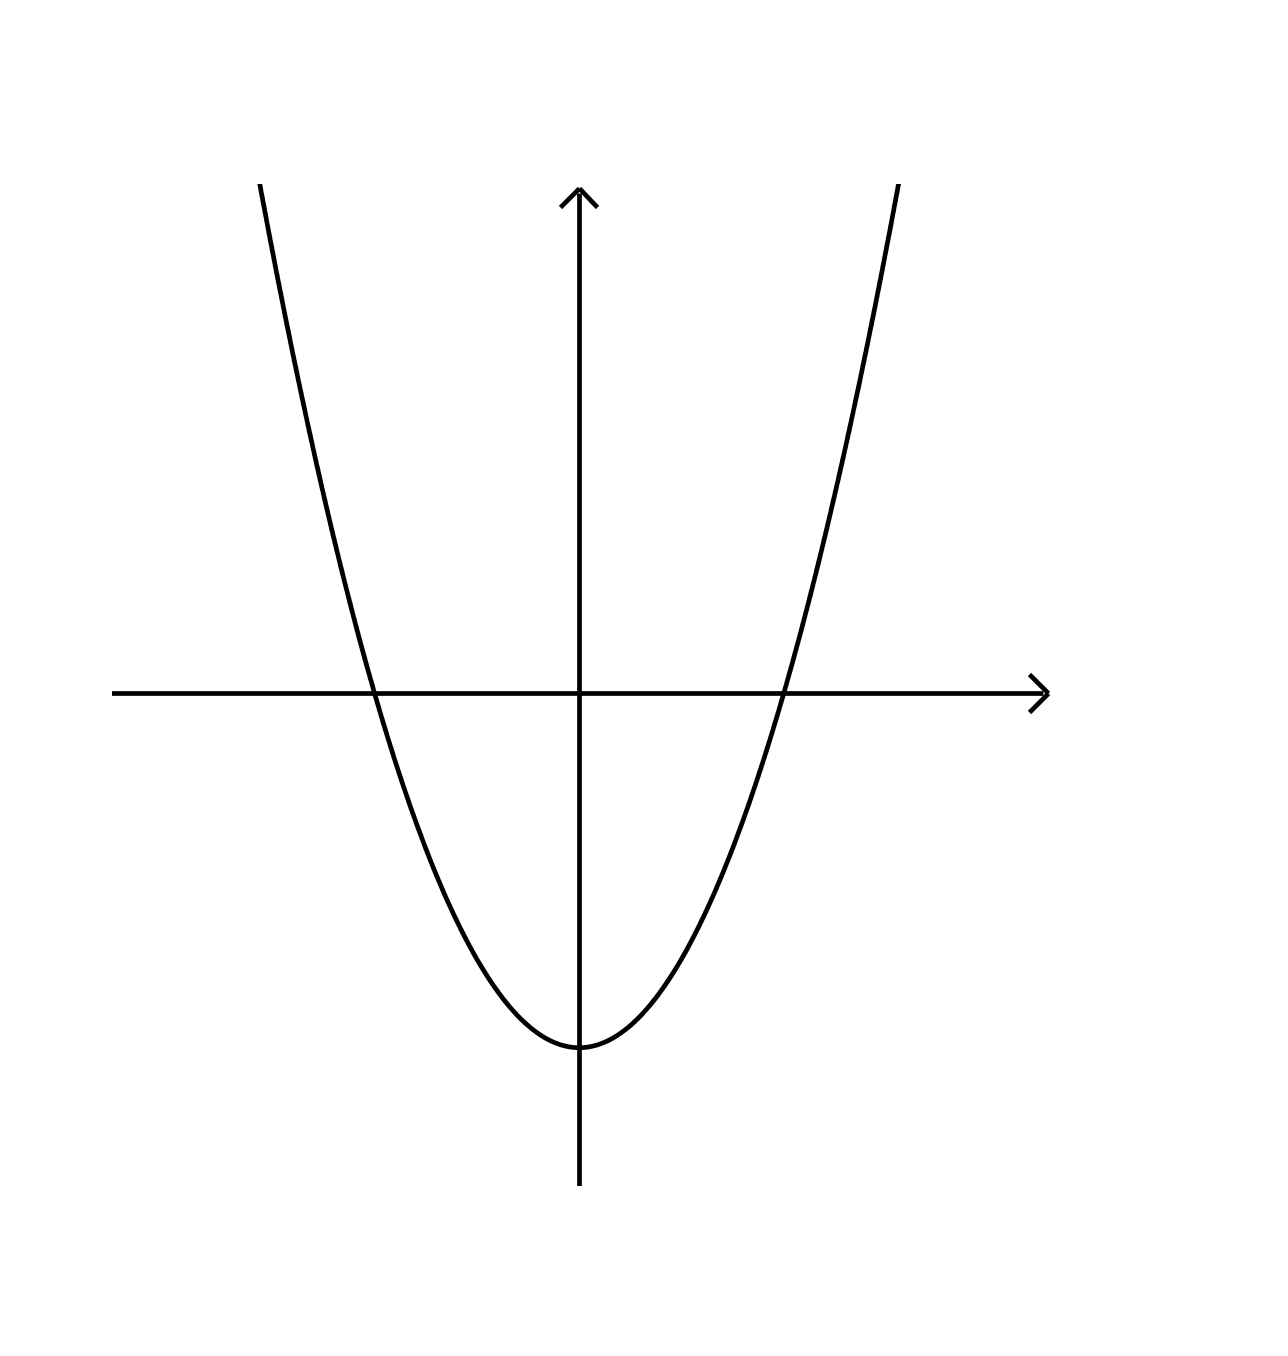
\includegraphics[width=0.4\textwidth]{graph_1}
~
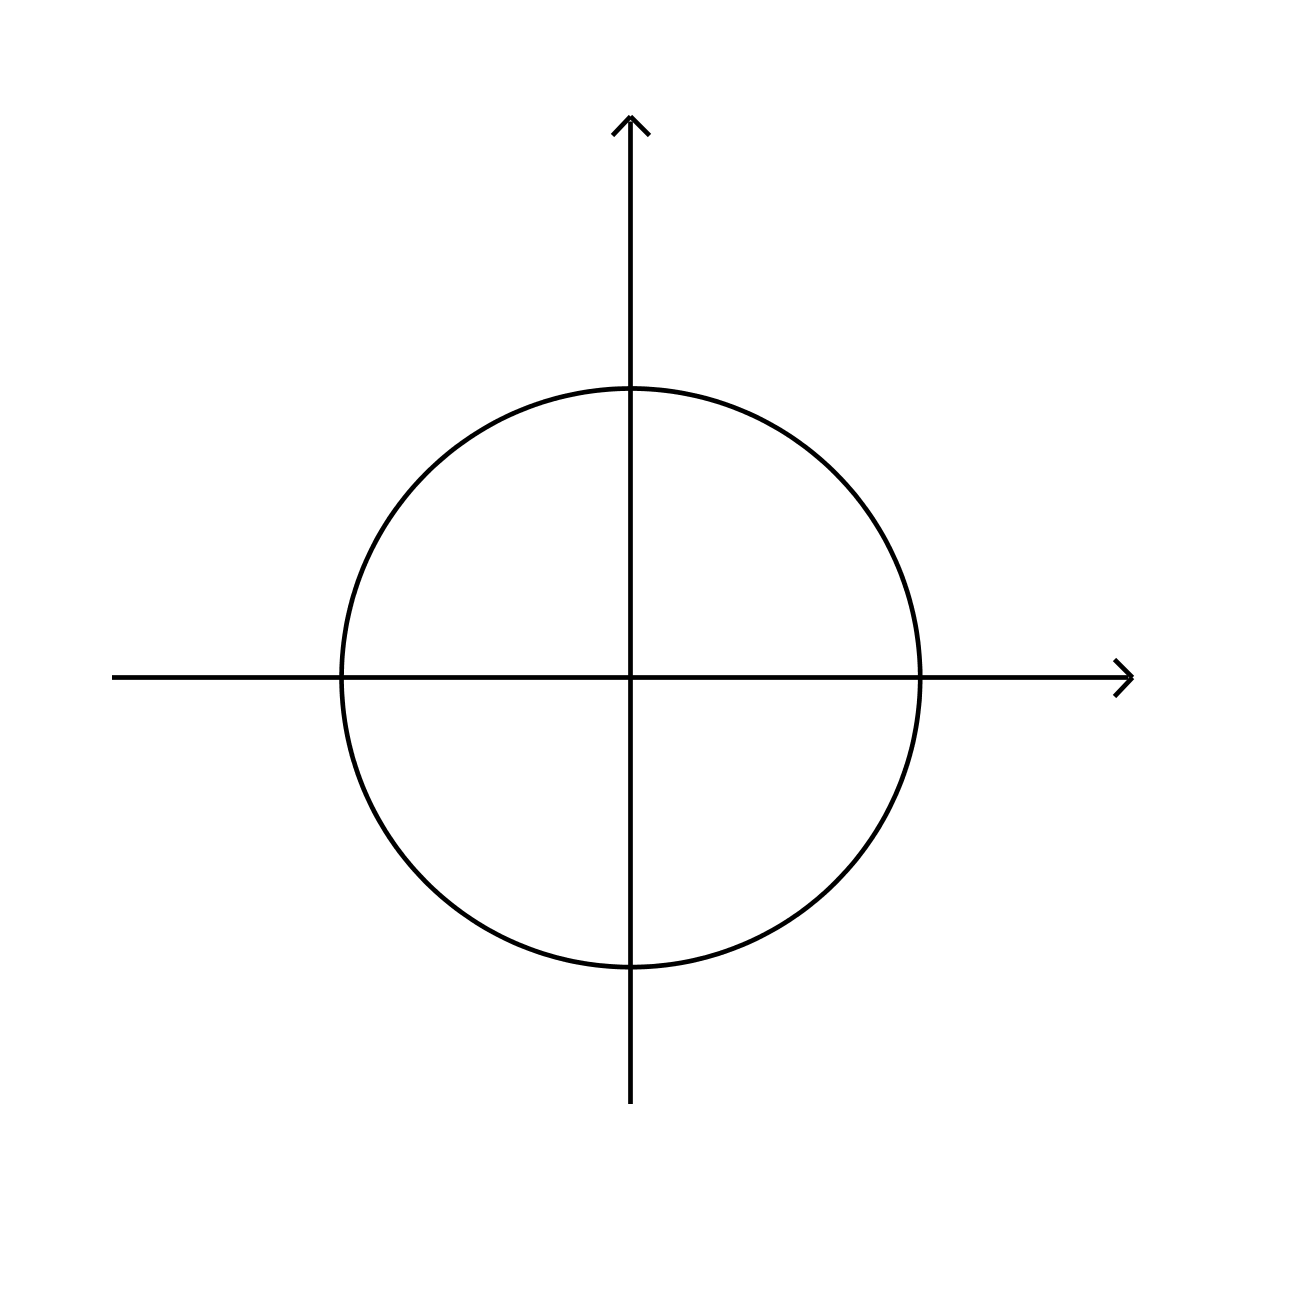
\includegraphics[width=0.4\textwidth]{graph_2}
\par\noindent(1)\qquad\qquad\qquad\qquad\qquad\qquad\qquad(2)\par\noindent
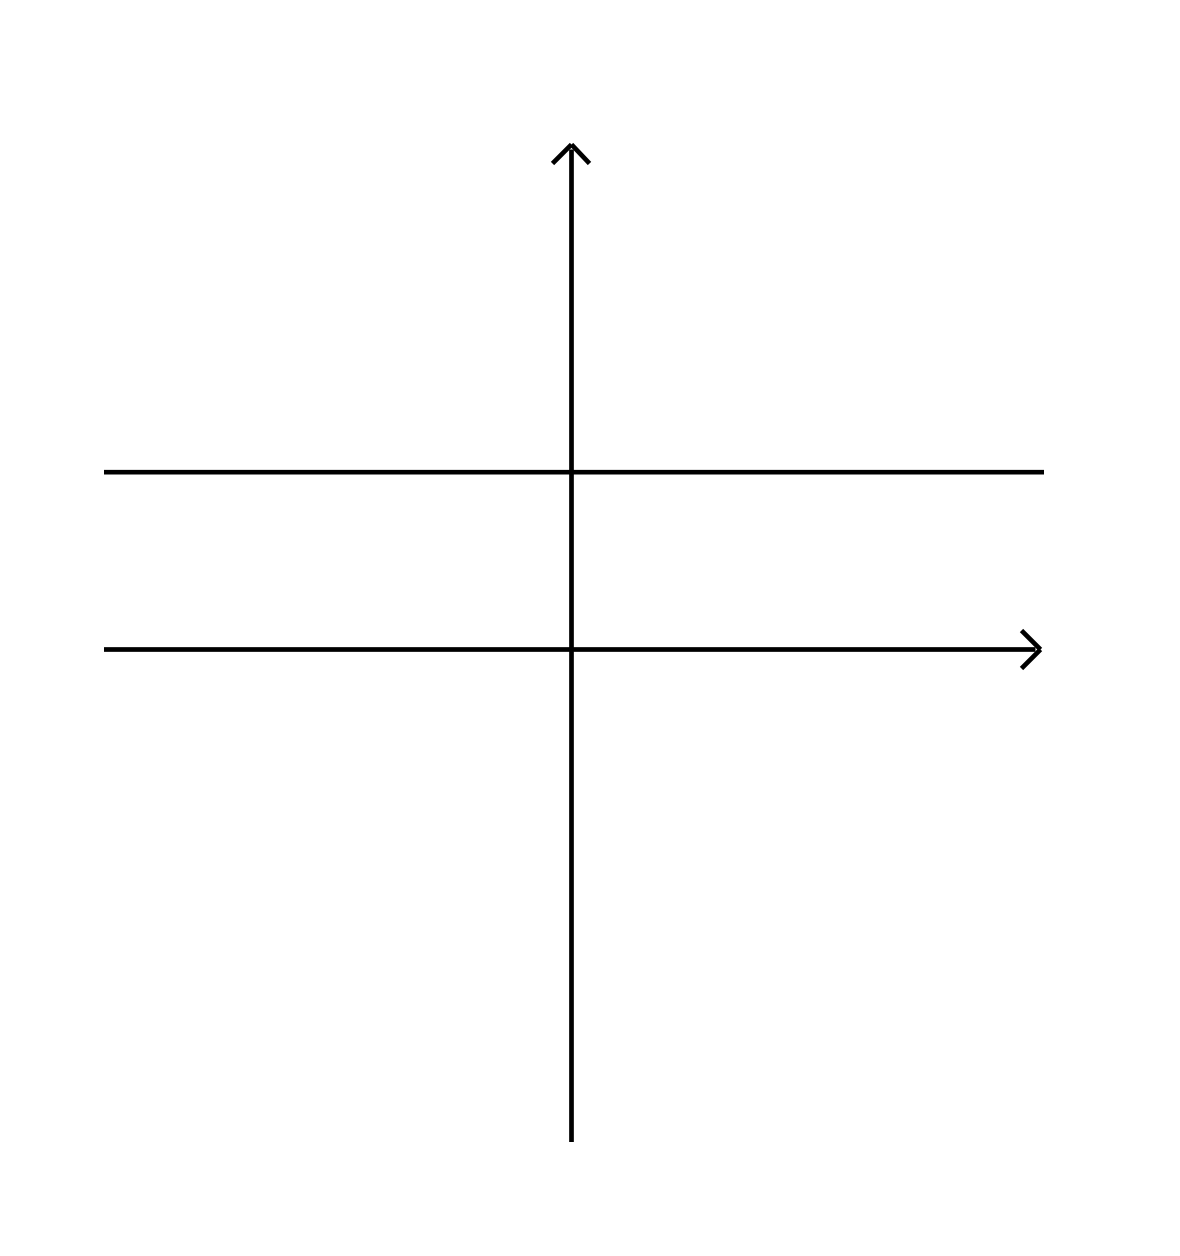
\includegraphics[width=0.4\textwidth]{graph_3}
~
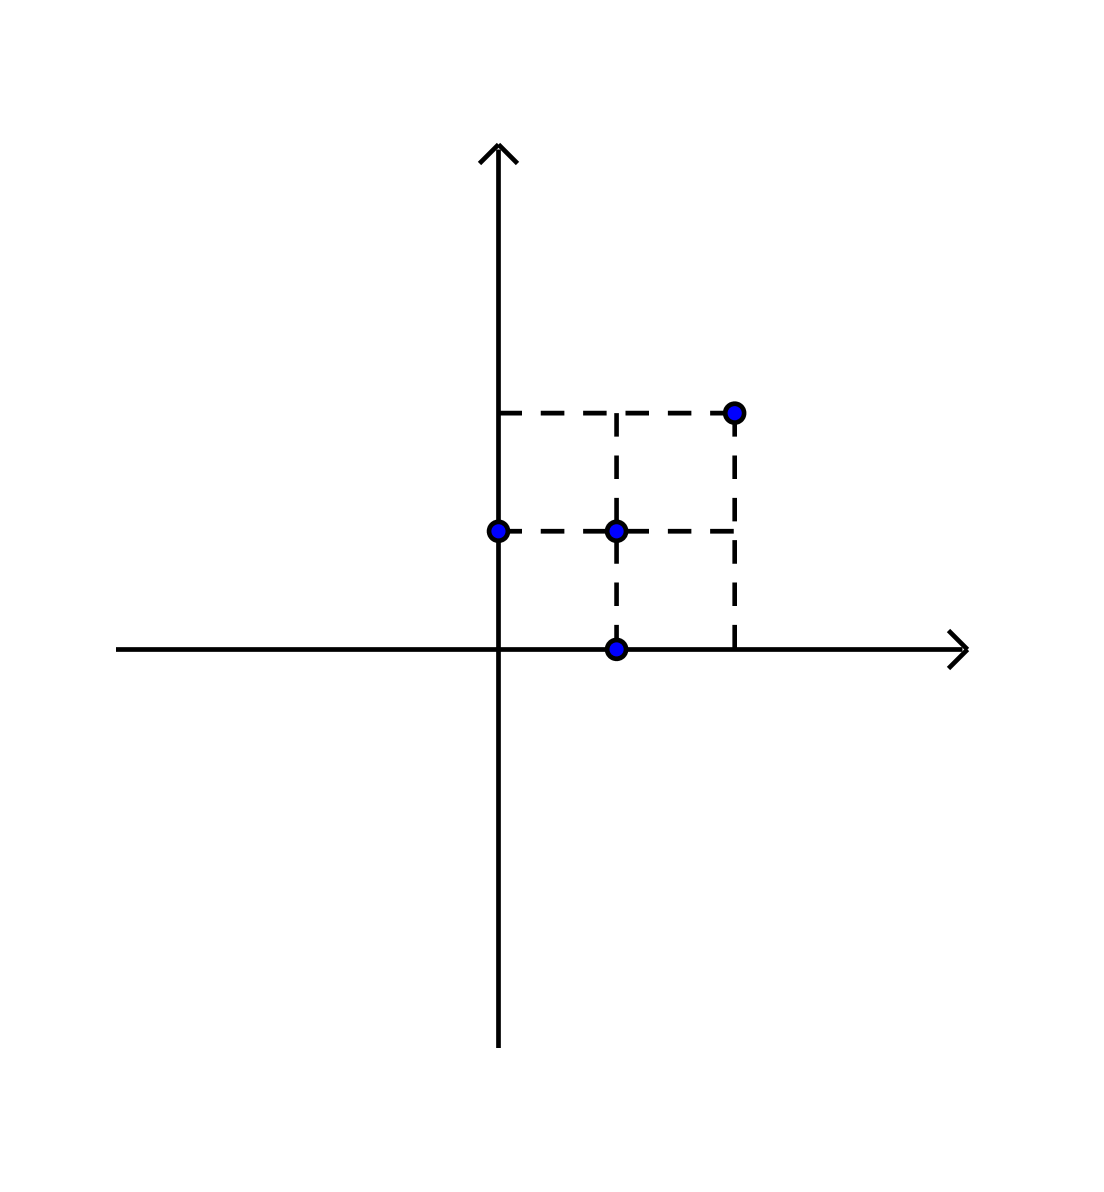
\includegraphics[width=0.4\textwidth]{graph_4}
\par\noindent(3)\qquad\qquad\qquad\qquad\qquad\qquad\qquad(4)
\end{figure}

%%
\section{여러 가지 함수}

\begin{mdframed}
%
\defi{}
함수 \(f:X\to Y\)에서
\[x_1\neq x_2\quad\Rightarrow\quad f(x_1)\neq f(x_2)\]
일 때, 혹은
\[f(x_1)=f(x_2)\quad\Rightarrow\quad x_1=x_2\]
일 때, 함수 \(f\)를 \emph{일대일 함수}라고 한다.
또한, 일대일 함수이면서 공역과 치역이 같은 함수를 \emph{일대일 대응}이라고 한다.
\end{mdframed}

%
\exam{}
\begin{figure}[h!]
\centering\noindent
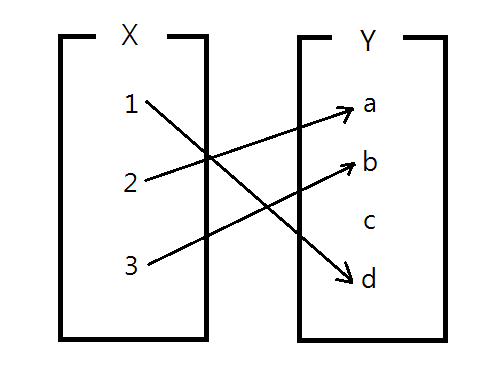
\includegraphics[width=0.3\textwidth]{injection_1}
~
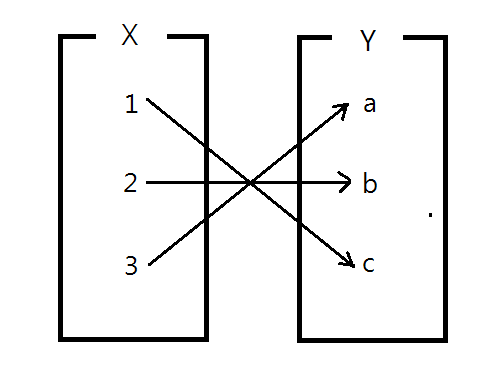
\includegraphics[width=0.3\textwidth]{injection_2}
~
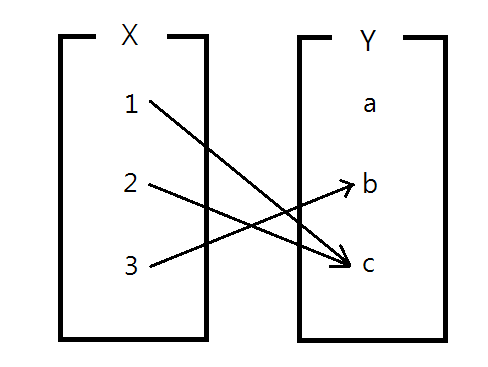
\includegraphics[width=0.3\textwidth]{injection_3}
\par\noindent(1)\qquad\qquad\qquad\qquad\qquad(2)\qquad\qquad\qquad\qquad\qquad(3)
\end{figure}

\begin{enumerate}
\item
각각의 \(x\)에 대한 함숫값 \(f(x)\)가 모두 다르다.
즉,
\[f(1)\neq f(2),\:\:f(2)\neq f(3),\:\:f(3)\neq f(1)\]
이다.
따라서 이 함수는 일대일 함수이다.
하지만 \(공역\neq치역\)이므로 일대일 대응은 아니다.
\item
마찬가지로 일대일 함수이다.
또 \(공역=치역\)이므로 일대일 대응이다.
\item
\(f(1)=f(2)\)이다.
즉, \(1\neq2\)임에도 불구하고 \(f(1)=f(2)\)이므로 일대일 함수가 아니고, 일대일 대응도 아니다.
\end{enumerate}

\clearpage
%
\exam{}
\begin{figure}[h!]
\centering\noindent
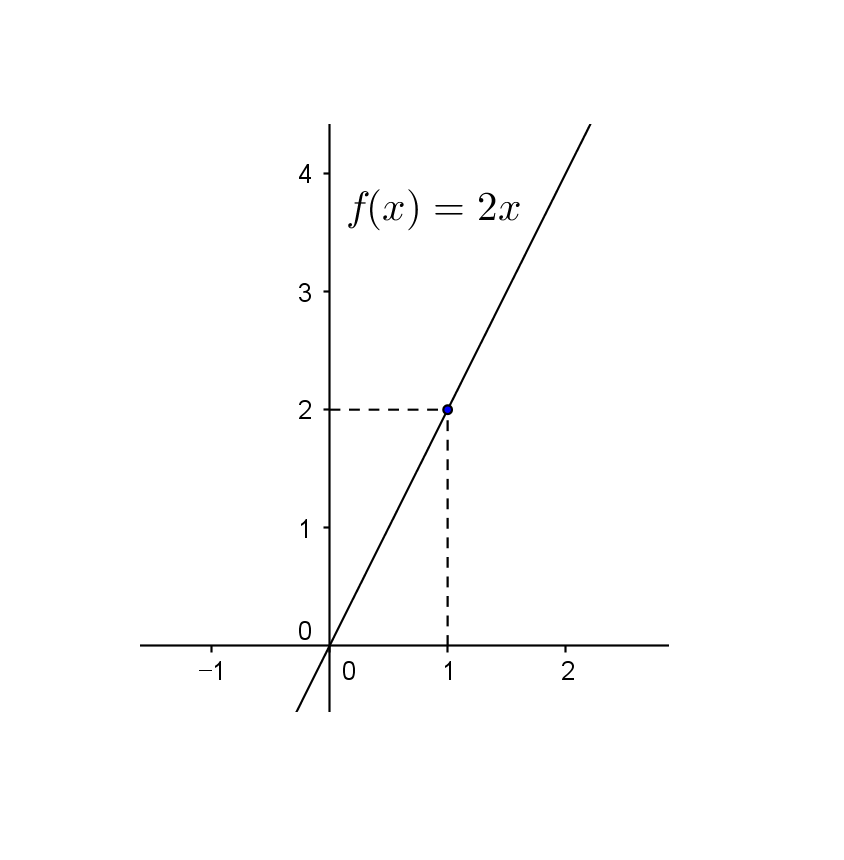
\includegraphics[width=0.4\textwidth]{injection_4}
~
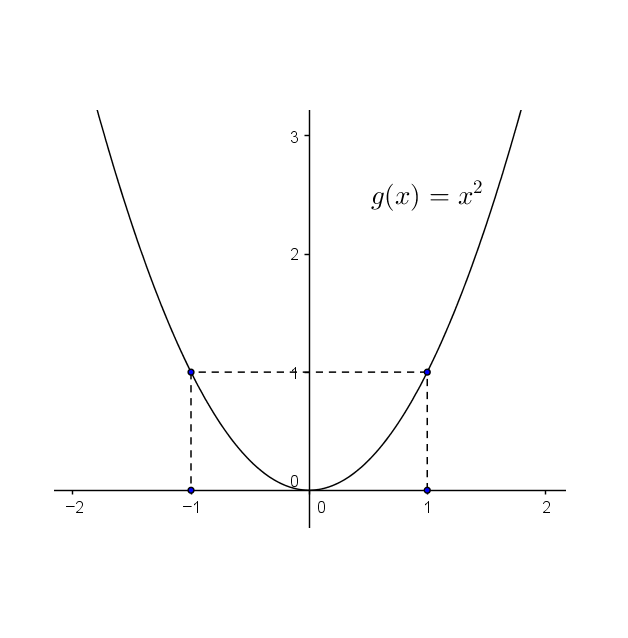
\includegraphics[width=0.4\textwidth]{injection_5}
\par\noindent(1)\qquad\qquad\qquad\qquad\qquad\qquad\qquad(2)
\end{figure}
\begin{enumerate}
\item
함수 \(f(x)=2x\)에서 \(f(x_1)=f(x_2)\)를 가정하면 \(2x_1=2x_2\)이므로 \(x_1=x_2\)이다.
따라서 \(f\)는 일대일 함수이다.
또한 치역이 실수 전체 집합으로, 공역과 같으므로 일대일 대응이기도 하다.%}
\item
함수 \(g(x)=x^2\)은 \(1\neq-1\)임에도 불구하고 \(f(1)=1=f(-1)\)이다.
따라서 \(g\) 일대일 함수가 아니고, 일대일 대응도 아니다.
\end{enumerate}

\prob{}
예시 \ref{nation1}, \ref{nation2}의 두 함수 중
\begin{figure*}[h!]
\centering
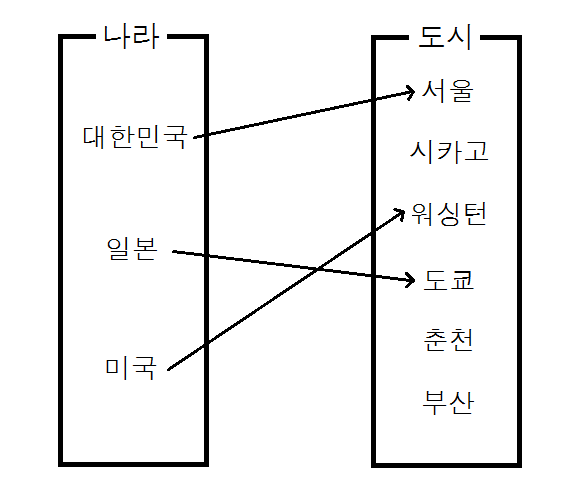
\includegraphics[width=0.3\textwidth]{nation-capital}
~
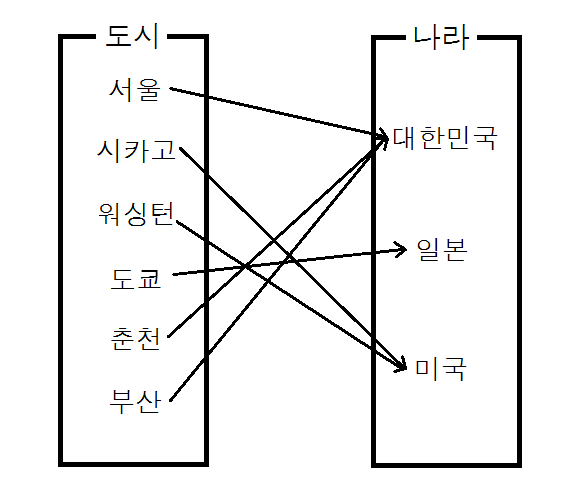
\includegraphics[width=0.3\textwidth]{city-nation}
\par\noindent
(1)
\qquad\qquad\qquad\qquad\quad\:\:
(2)
\end{figure*}

첫번째 함수는
\tabto{0.25\textwidth}(일대일 함수이다, 일대일 함수가 아니다.)\\
\tabto{0.25\textwidth}(일대일 대응이다, 일대일 대응이 아니다.)

두 번째 함수는
\tabto{0.25\textwidth}(일대일 함수이다, 일대일 함수가 아니다.)\\
\tabto{0.25\textwidth}(일대일 대응이다, 일대일 대응이 아니다.)

\clearpage
%
\prob{}
다음 함수들의 그래프를 그리고 일대일 함수와 일대일 대응을 찾아라.
\par\noindent
(1)\:\:\(y=2x+4\)
\tabto{.5\textwidth}
(2)\:\:\(y=|x|\)
\par\noindent
(3)\:\:\(y=x^2-1\) (\(x\ge0\))
\tabto{.5\textwidth}
(4)\:\:\(y=2\)

\textbf{답 :}
\begin{figure*}[h!]
\centering
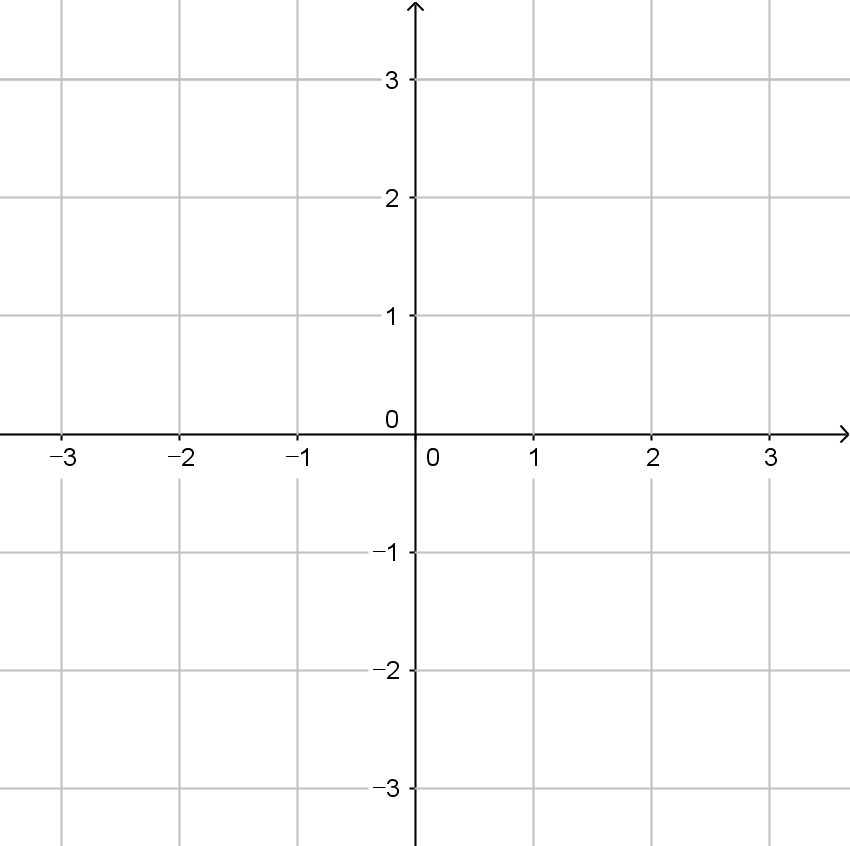
\includegraphics[width=0.28\textwidth]{pm3by3}
~
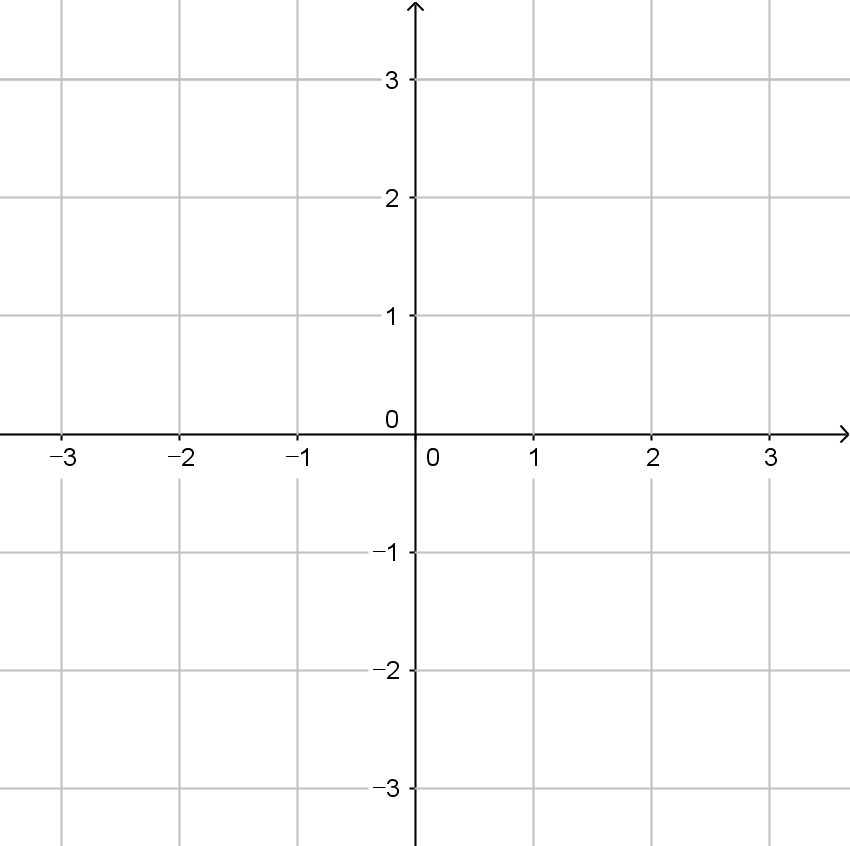
\includegraphics[width=0.28\textwidth]{pm3by3}
\par\noindent
(1)
\qquad\qquad\qquad\qquad\quad
(2)
\par\noindent
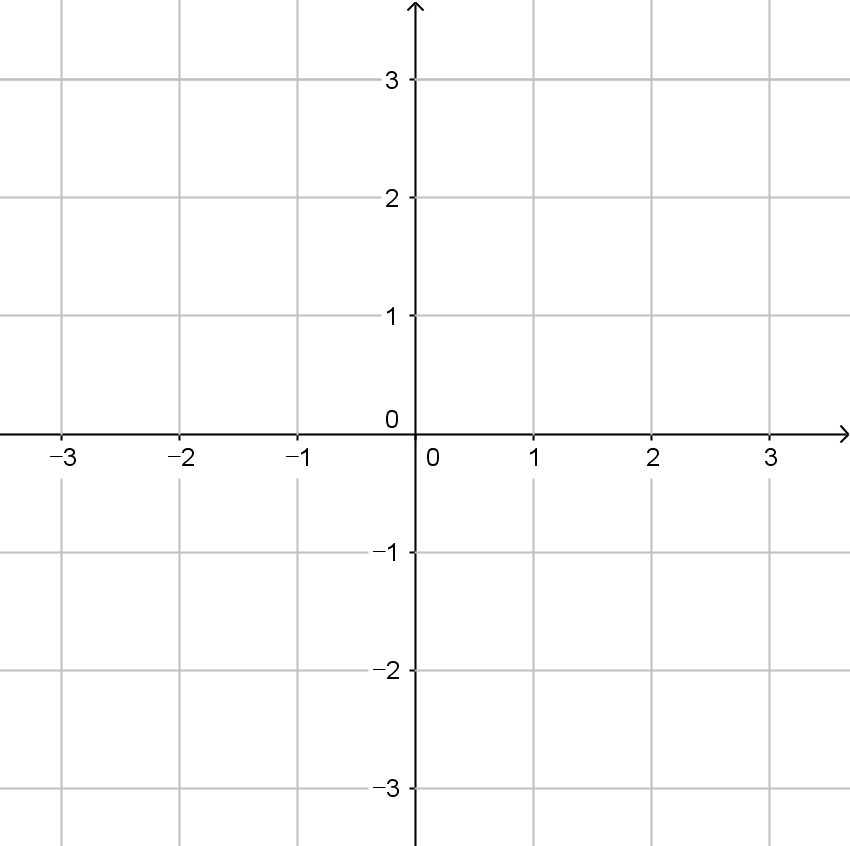
\includegraphics[width=0.28\textwidth]{pm3by3}
~
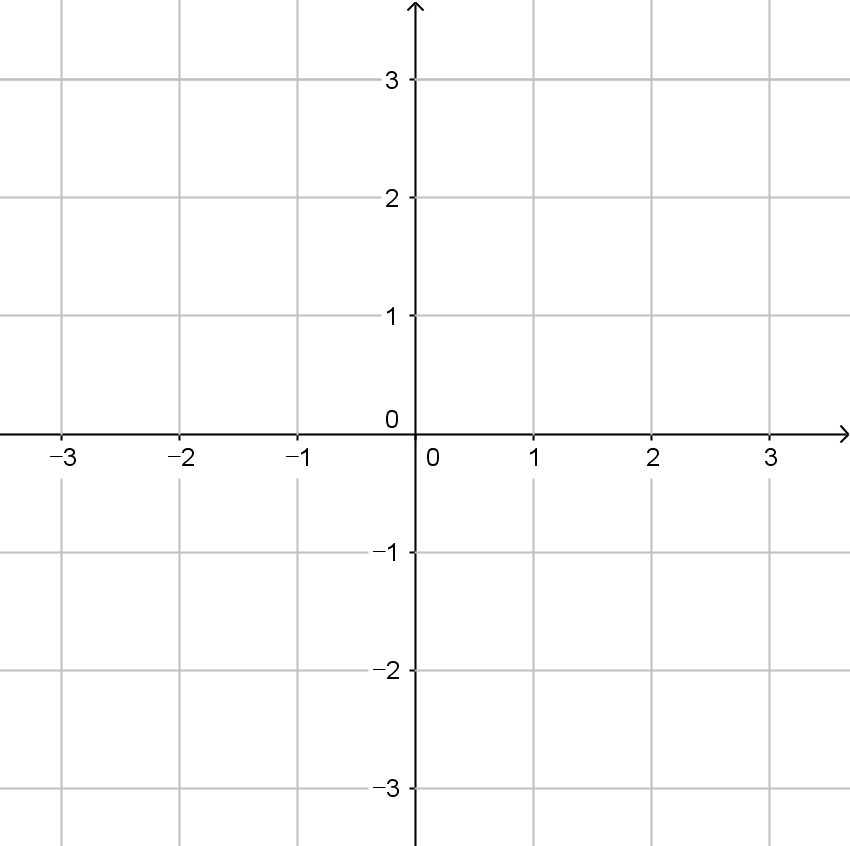
\includegraphics[width=0.28\textwidth]{pm3by3}
\par\noindent
(3)
\qquad\qquad\qquad\qquad\quad
(4)
\end{figure*}

\prob{}
\begin{enumerate}
\item
함수 \(y=3x-2\)가 일대일 함수임을 증명하여라.
\item
함수 \(y=x^2-5\)가 일대일 함수가 아님을 증명하여라.
\end{enumerate}
\procedure{0.2}

\clearpage
\begin{mdframed}
%
\defi{}
정의역과 공역이 같은 함수 \(f:X\to X\)에서, 모든 \(x\in X\)에 대해
\[f(x)=x\]
일 때, 함수 \(f\)를 \emph{항등함수}라고 한다.
항등함수는 보통 \(I\)로 쓴다.
정의역과 공역을 강조하기 위해 \(I_X\)라고 쓰기도 한다.

또, 함수 \(f:X\to Y\)에서, \(c\)가 \(Y\)의 원소일 때, 모든 \(x\in X\)에 대해
\[f(x)=c\]
일 때, 함수 \(f\)를 \emph{상수함수}라고 한다.
\end{mdframed}

%
\exam{}
\begin{figure}[h!]
\centering\noindent
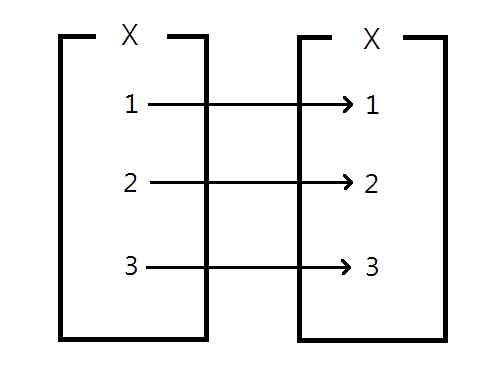
\includegraphics[width=0.4\textwidth]{identity}
~
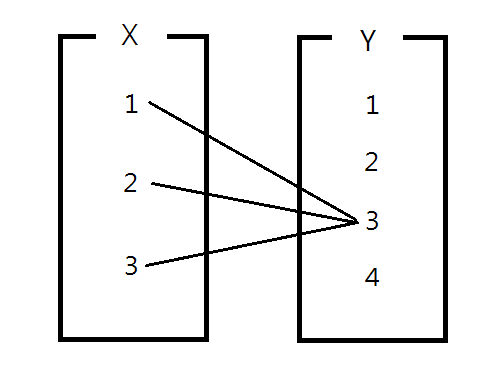
\includegraphics[width=0.4\textwidth]{constant}
\par\noindent(1)\qquad\qquad\qquad\qquad\qquad(2)
\end{figure}

\begin{enumerate}
\item
\(f(1)=1\), \(f(2)=2\), \(f(3)=3\)이므로 모든 \(x\in X\)에 대해 \(f(x)=x\)이다.
따라서 \(f\)는 항등함수이고 \(f=I\) 혹은 \(f=I_X\)라고 쓸 수 있다.
\item
\(f(1)=3\), \(f(2)=3\), \(f(3)=3\)이므로 모든 \(x\in X\)에 대해 \(f(x)=3\)이다.
따라서 \(f\)는 상수함수이다.
\end{enumerate}

%
\prob{}
다음 함수 중 항등함수와 상수함수를 찾아라.
\par\noindent
(1)\:\:\(y=x\)
\tabto{0.49\textwidth}
(2)\:\:\(y=-1\)
\par\noindent
(3)\:\:\(y=2x\)
\tabto{0.49\textwidth}
(4)\:\:\(y=x^2\)
%\begin{enumerate}
%\item
%\(y=x\)
%\item
%\(y=-1\)
%\item
%\(y=2x\)
%\item
%\(y=x^2\)
%\end{enumerate}

%%
\section{보충 · 심화문제}

\prob{}
다음 함수들의 그래프를 그려라.
\begin{figure*}[h!]
\centering
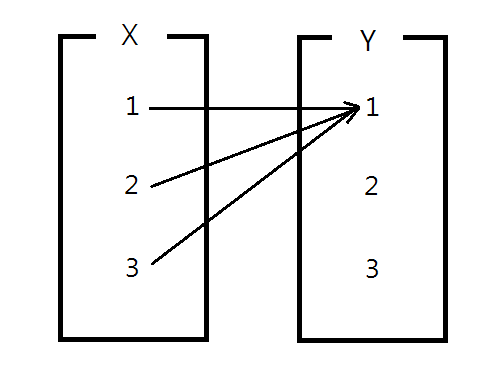
\includegraphics[width=0.28\textwidth]{function-1}
~
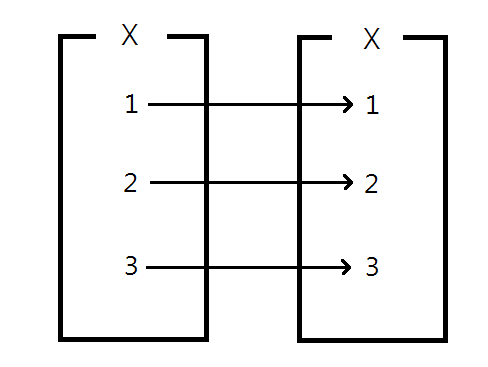
\includegraphics[width=0.28\textwidth]{function-2}
\par\noindent
(1)
\qquad\qquad\qquad\qquad\quad
(2)
\par\noindent
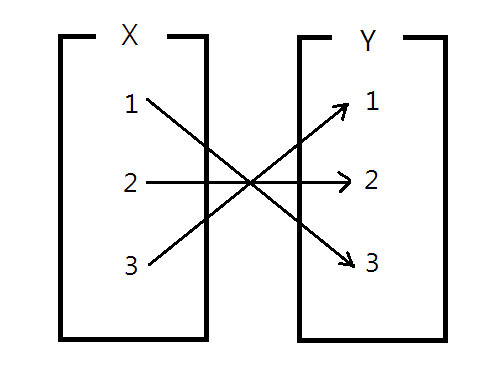
\includegraphics[width=0.28\textwidth]{function-3}
~
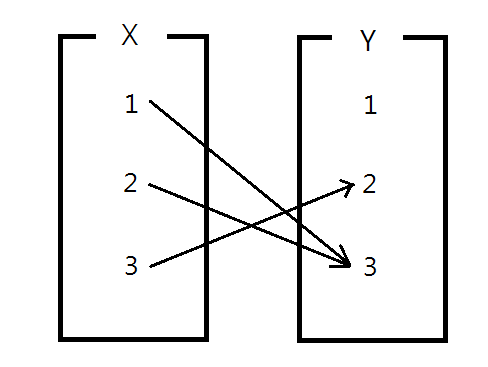
\includegraphics[width=0.28\textwidth]{function-4}
\par\noindent
(3)
\qquad\qquad\qquad\qquad\quad
(4)
\end{figure*}

\textbf{답 :}
\begin{figure*}[h!]
\centering
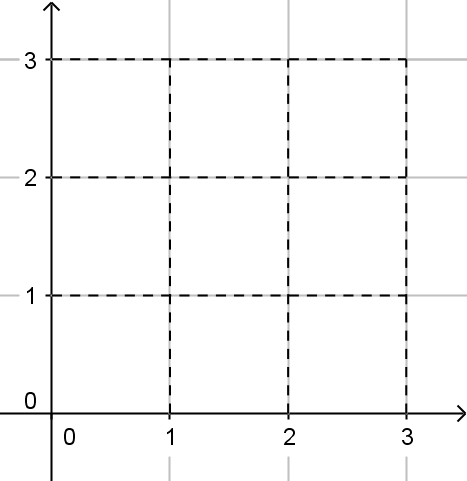
\includegraphics[width=0.28\textwidth]{3by3}
~
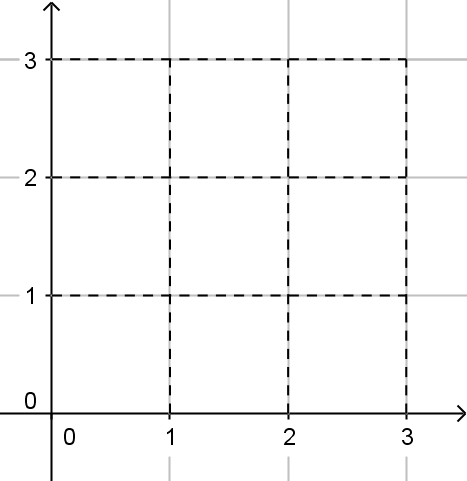
\includegraphics[width=0.28\textwidth]{3by3}
\par\noindent
(1)
\qquad\qquad\qquad\qquad\quad
(2)
\par\noindent
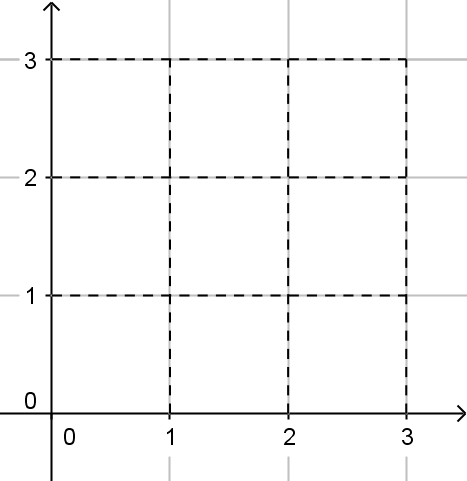
\includegraphics[width=0.28\textwidth]{3by3}
~
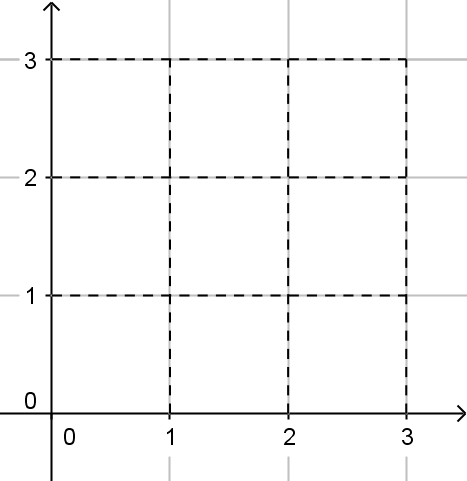
\includegraphics[width=0.28\textwidth]{3by3}
\par\noindent
(3)
\qquad\qquad\qquad\qquad\quad
(4)
\end{figure*}

\prob{}
다음 함수들의 그래프를 그리고, 정의역과 치역을 각각 구하여라.
\par\noindent
(1)\:\:\(y=x+2\)
\tabto{.5\textwidth}
(2)\:\:\(y=2-x^2\)
\par\noindent
(3)\:\:\(y=\frac2x\)
\tabto{.5\textwidth}
(4)\:\:\(y=\sqrt{4-x^2}\)

\textbf{답 :}
\begin{figure*}[h!]
\centering
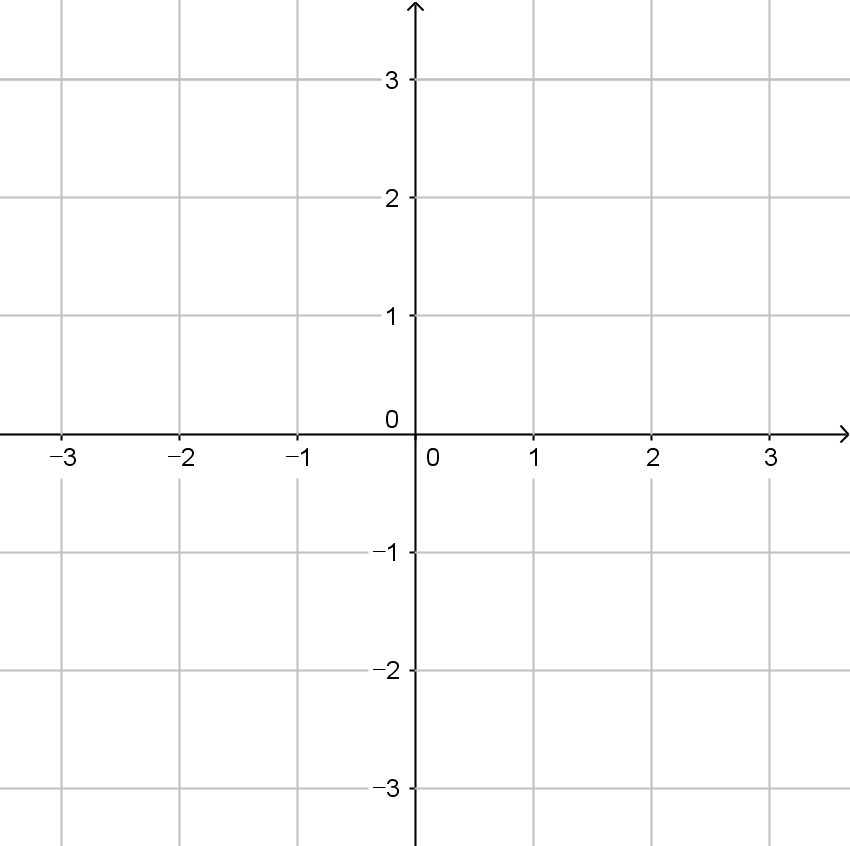
\includegraphics[width=0.28\textwidth]{pm3by3}
~
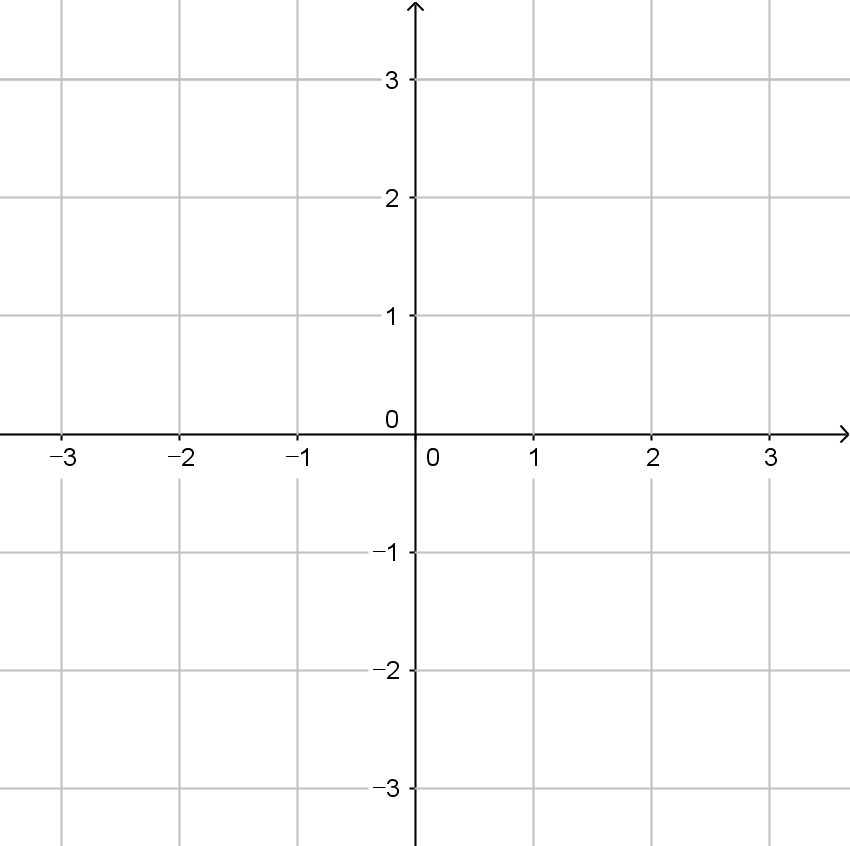
\includegraphics[width=0.28\textwidth]{pm3by3}
\par\noindent
(1)
\qquad\qquad\qquad\qquad\quad
(2)
\par\noindent
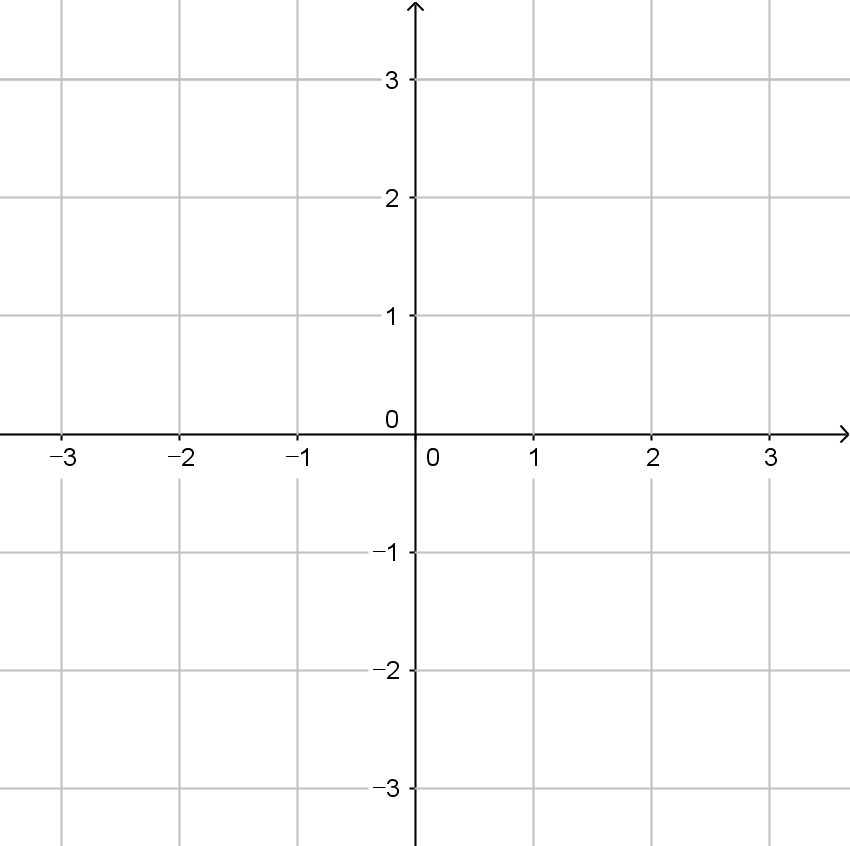
\includegraphics[width=0.28\textwidth]{pm3by3}
~
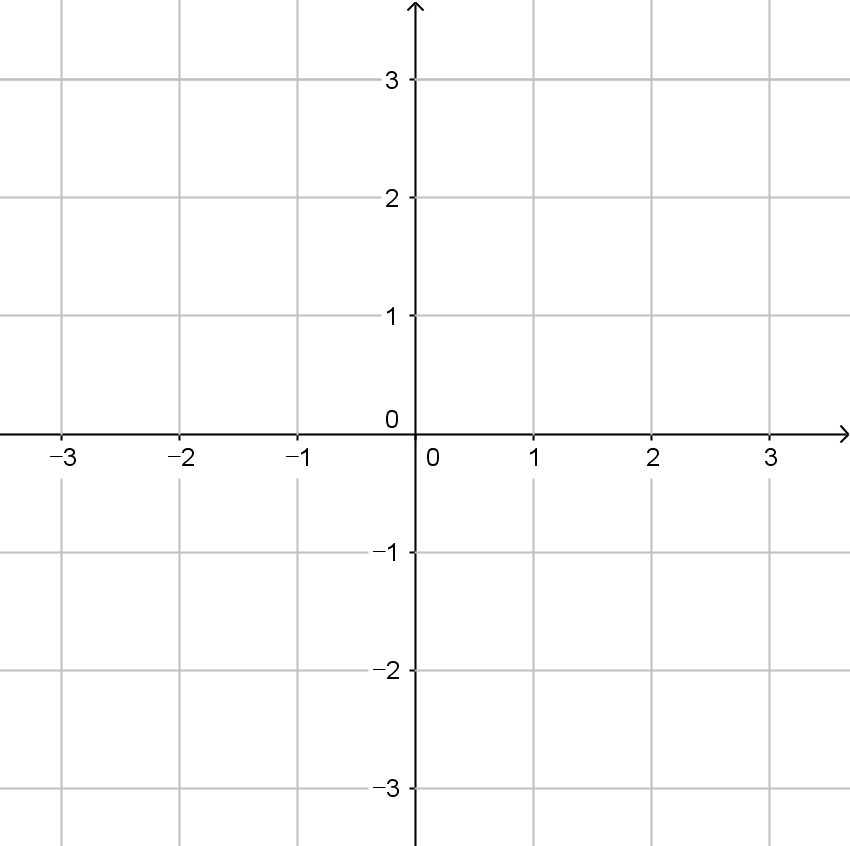
\includegraphics[width=0.28\textwidth]{pm3by3}
\par\noindent
(3)
\qquad\qquad\qquad\qquad\quad
(4)
\end{figure*}
\begin{enumerate}
\item
정의역=\phantom{실수 전체 집합}, 치역=\phantom{실수 전체 집합}
\item
정의역=\phantom{실수 전체 집합}, 치역=\phantom{실수 전체 집합}
\item
정의역=\phantom{실수 전체 집합}, 치역=\phantom{실수 전체 집합}
\item
정의역=\phantom{실수 전체 집합}, 치역=\phantom{실수 전체 집합}
\end{enumerate}

\clearpage
%
\prob{}
다음 두 집합 \(X\), \(Y\)에 대하여 \(X\)에서 \(Y\)로의 함수 \(f(x)=ax+b\)가 일대일 대응이 되도록 두 실수 \(a\), \(b\)의 값을 정하여라.
\[X=\{x\ba1\le x\le3\},\quad Y=\{y\ba-1\le y\le5\}\]
\ans
\vspace{0.2\textheight}

%
\prob{}
두 집합 \(X=\{x\ba x\text{는 }2\le x\le15\text{인 자연수}\}\), \(Y=\{y\ba y\text{는 자연수}\}\)에 대하여 함수 \(f:X\to Y\), \(f(x)=(x\text{의 양의 약수의 개수})\)일 때, \(f(x)=3\)을 만족하는 \(x\)의 값을 모두 구하여라.
\ans
\vspace{0.2\textheight}


%%
\section*{답}

\begin{minipage}{0.49\textwidth}
%
\an{5}
\begin{enumerate}[topsep=0pt]
\item
함수이다.\\
\(정의역=\{a,b,c\}\),\\
\(공역=\{1,2,3\}\),\\
\(치역=\{1\}\)
\item
함수가 아니다.
\item
함수가 아니다.
\end{enumerate}

%
\an{7}
\begin{enumerate}[topsep=0pt]
\item
정의역=실수 전체 집합,\\
치역=실수 전체 집합
\item
정의역=실수 전체 집합,\\
치역=\(\{y\ba y\ge-3\}\)
\item
정의역=\(\{x\ba x\neq0\}\),\\
치역=\(\{y\ba y\neq0\}\)
\item
정의역=실수 전체 집합,\\
치역=\(\{4\}\)
\end{enumerate}

%
\an{10}
(1) 같다,\qquad
(2) 다르다.

%
\an{16}
(1), (3)
\end{minipage}
%%%%
\begin{minipage}{0.49\textwidth}
\an{20}
일대일 함수이다,\\
일대일 대응이 아니다.\\
일대일 함수가 아니다,\\
일대일 대응이 아니다.

%
\an{21}
\begin{center}
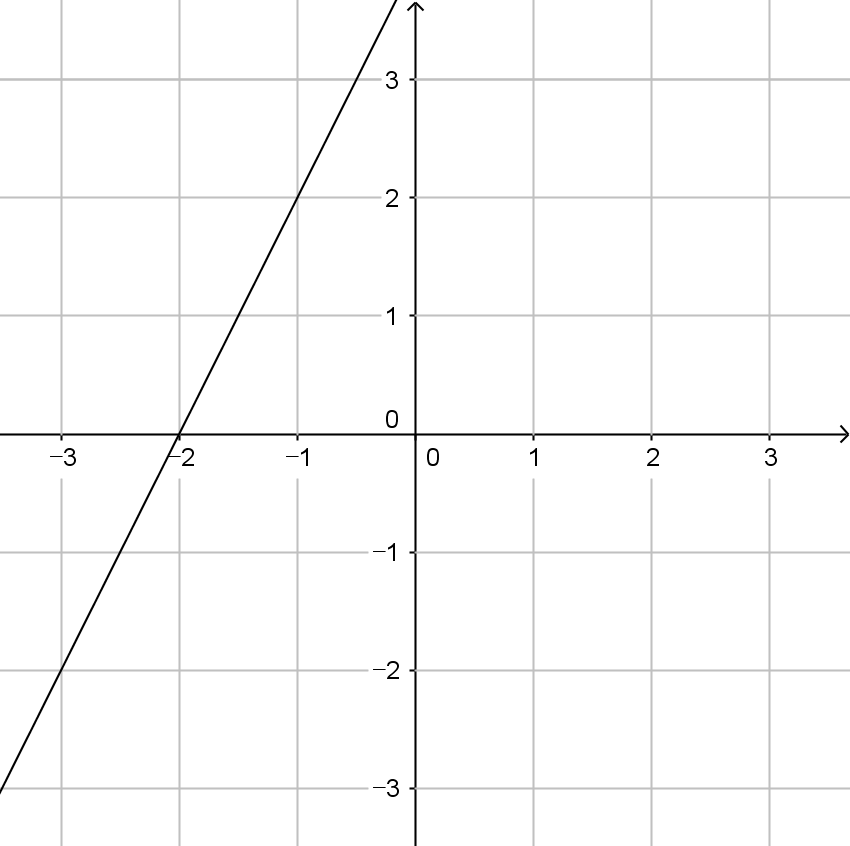
\includegraphics[width=0.45\textwidth]{pm3by3_y=2x+4}
~
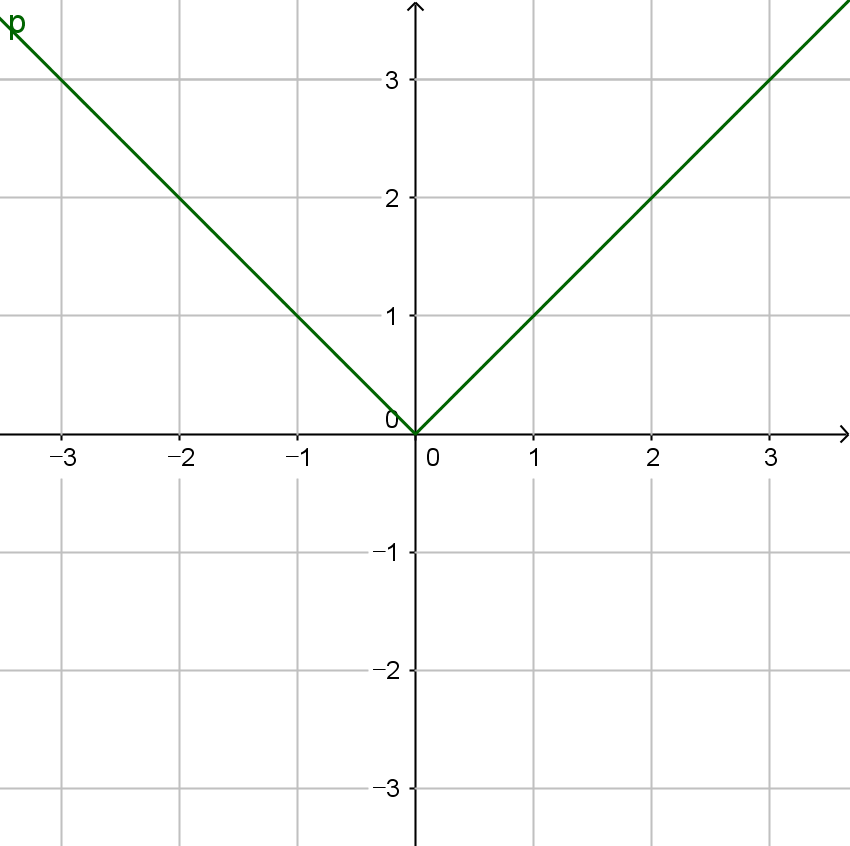
\includegraphics[width=0.45\textwidth]{pm3by3_absx}
\par\noindent(1)\qquad\qquad\qquad\quad\:\:(2)\par\noindent
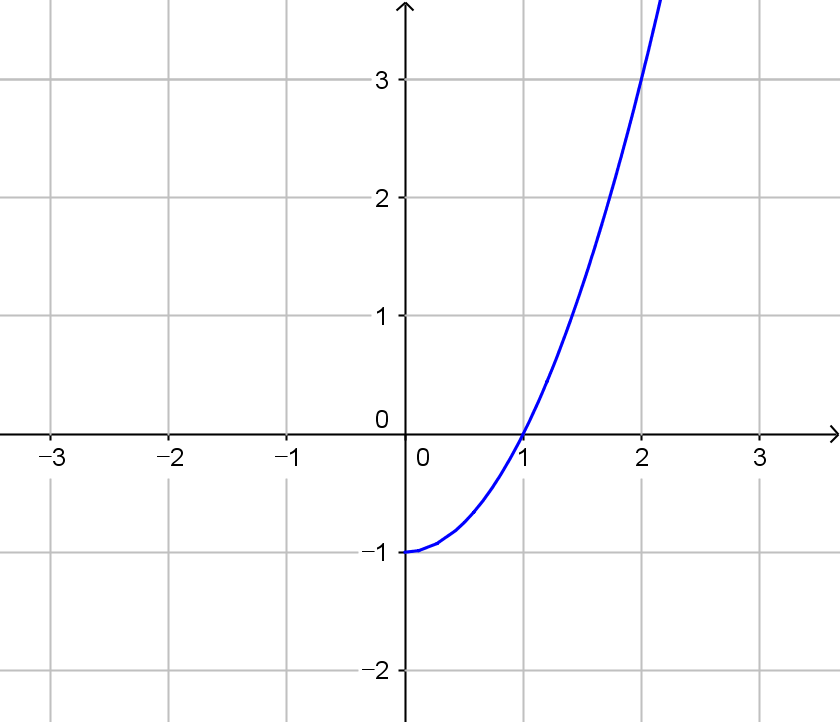
\includegraphics[width=0.45\textwidth]{pm3by3_x^2-1}
~
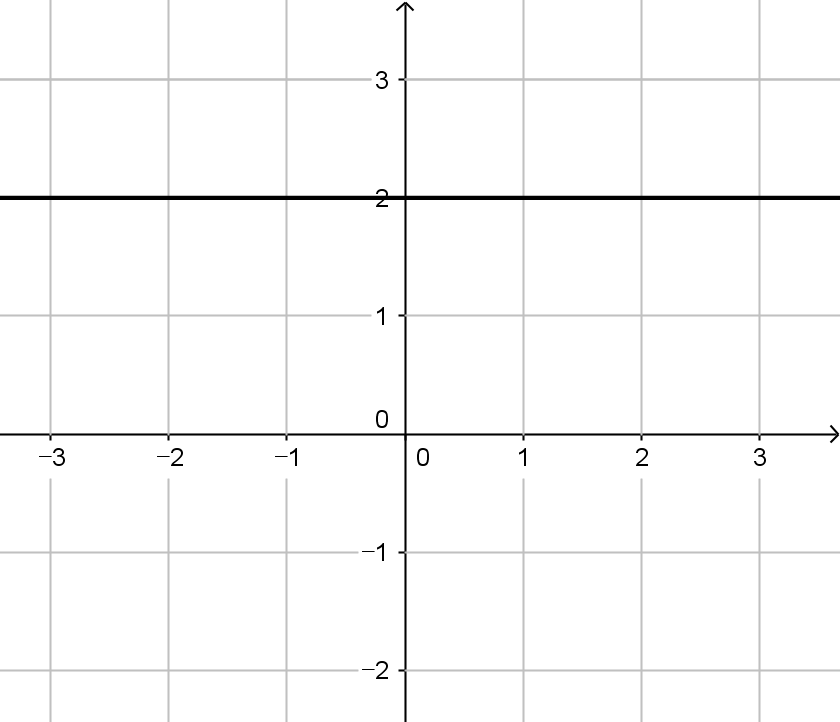
\includegraphics[width=0.45\textwidth]{pm3by3_y=2}
\par\noindent(3)\qquad\qquad\qquad\quad\:\:(4)
\end{center}
\begin{enumerate}[topsep=0pt]
\item
일대일 함수이면서 일대일 대응이다.
\item
일대일 함수도, 일대일 대응도 아니다.
\item
일대일 함수이지만 일대일 대응은 아니다.
\item
일대일 함수도, 일대일 대응도 아니다.
\end{enumerate}
\end{minipage}

\begin{minipage}{0.49\textwidth}
%
\an{22}
\begin{enumerate}[topsep=0pt]
\item
\(f(x)=3x-2\)라고 하자.\\
\(f(x_1)=f(x_2)\)를 가정하면,\\ \(3x_1-2=3x_2-2\)이다.\\
따라서 \(x_1=x_2\)이다.
\[f(x_1)=f(x_2)\quad\Rightarrow\quad x_1=x_2\]
이므로 \(f\)는 일대일 함수이다.
\item
\(g(x)=x^2-5\)라고 하자.
\(2\neq-2\)이지만 \(g(2)=-1=g(-2)\)이다.
따라서 \(g\)는 일대일 함수가 아니다.
\end{enumerate}

%
\an{25}
항등함수 : (1)\\ 상수함수 : (2)

%
\an{26}
\begin{center}
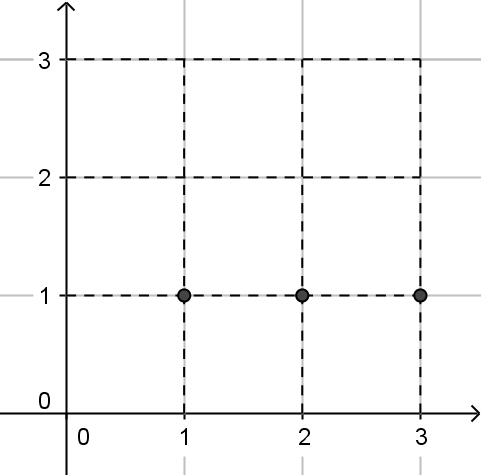
\includegraphics[width=0.45\textwidth]{3by3_1}
~
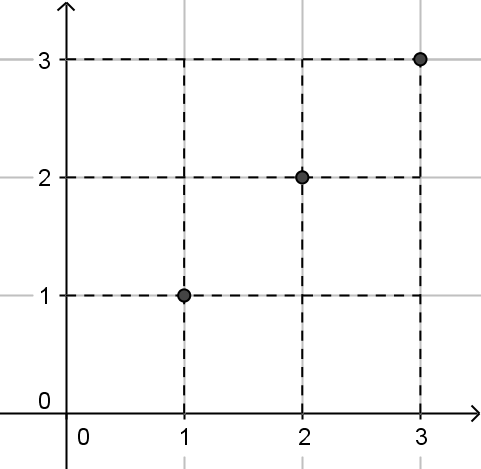
\includegraphics[width=0.45\textwidth]{3by3_2}
\par\noindent(1)\qquad\qquad\qquad\quad\:\:(2)\par\noindent
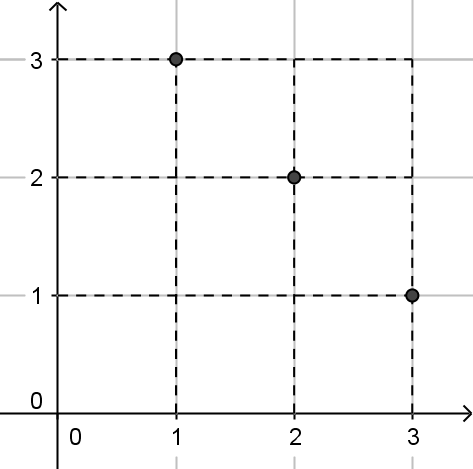
\includegraphics[width=0.45\textwidth]{3by3_3}
~
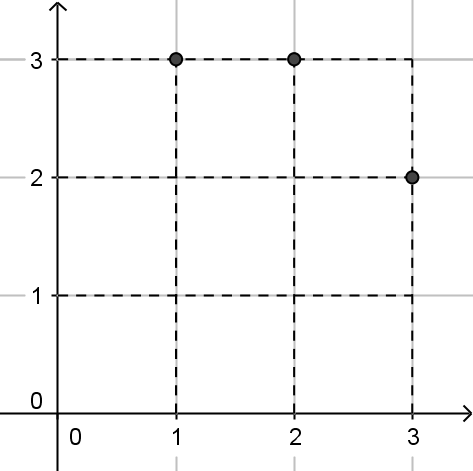
\includegraphics[width=0.45\textwidth]{3by3_4}
\par\noindent(3)\qquad\qquad\qquad\quad\:\:(4)
\end{center}
\end{minipage}
%%%
\begin{minipage}{0.49\textwidth}
%
\an{27}
\begin{center}
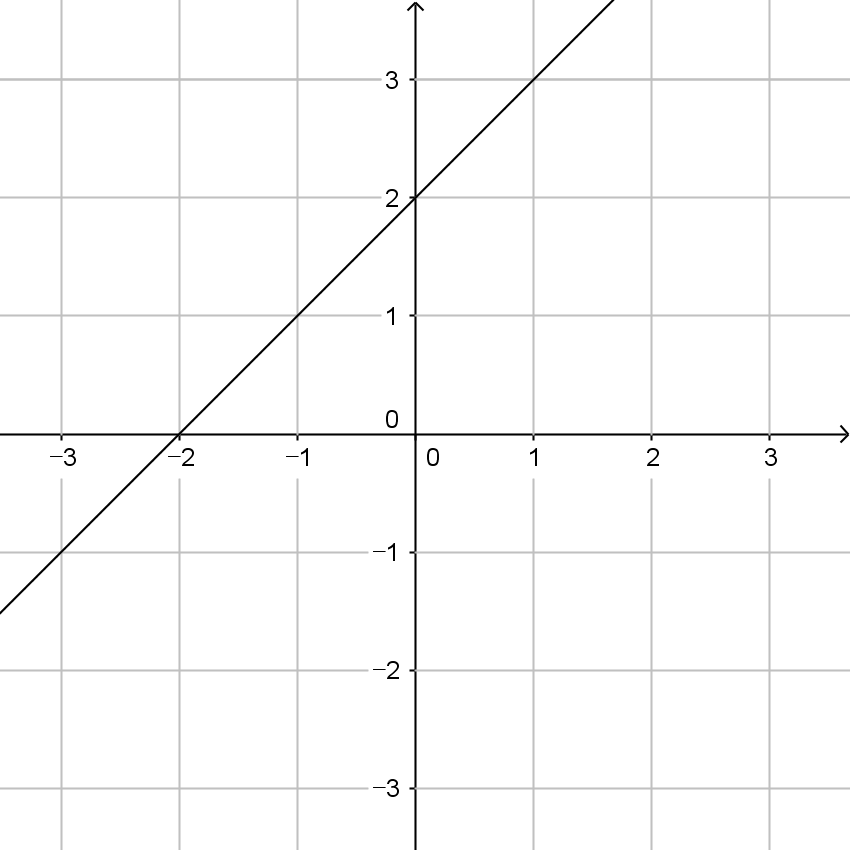
\includegraphics[width=0.45\textwidth]{pm3by3_y=x+2}
~
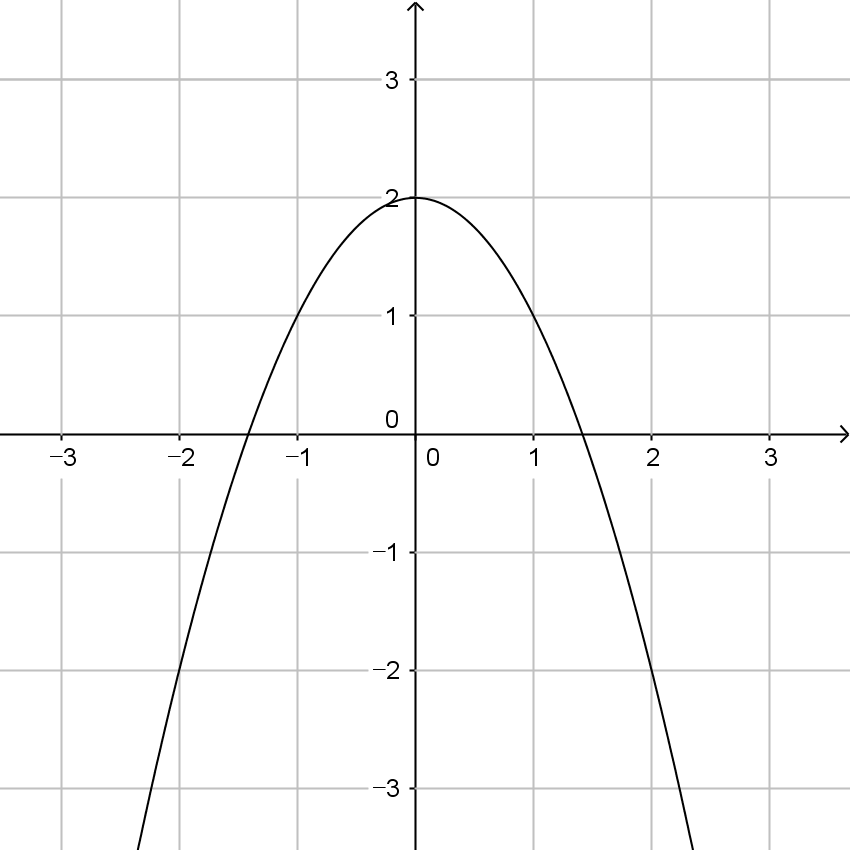
\includegraphics[width=0.45\textwidth]{pm3by3_y=2-x^2}
\par\noindent(1)\qquad\qquad\qquad\quad\:\:(2)\par\noindent
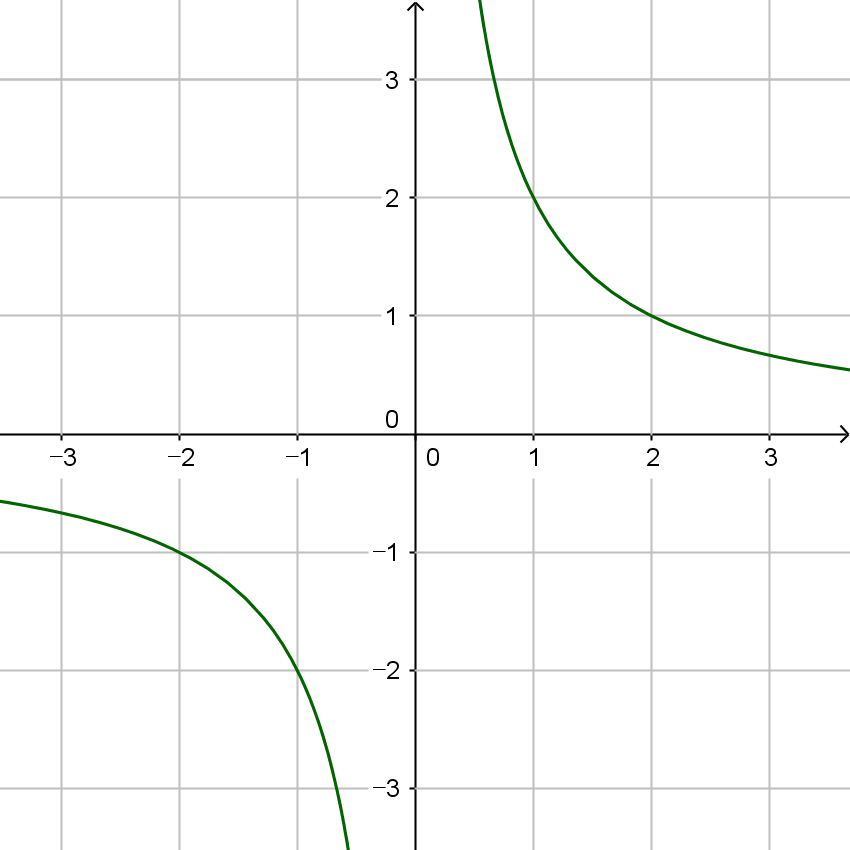
\includegraphics[width=0.45\textwidth]{pm3by3_y=frac2x}
~
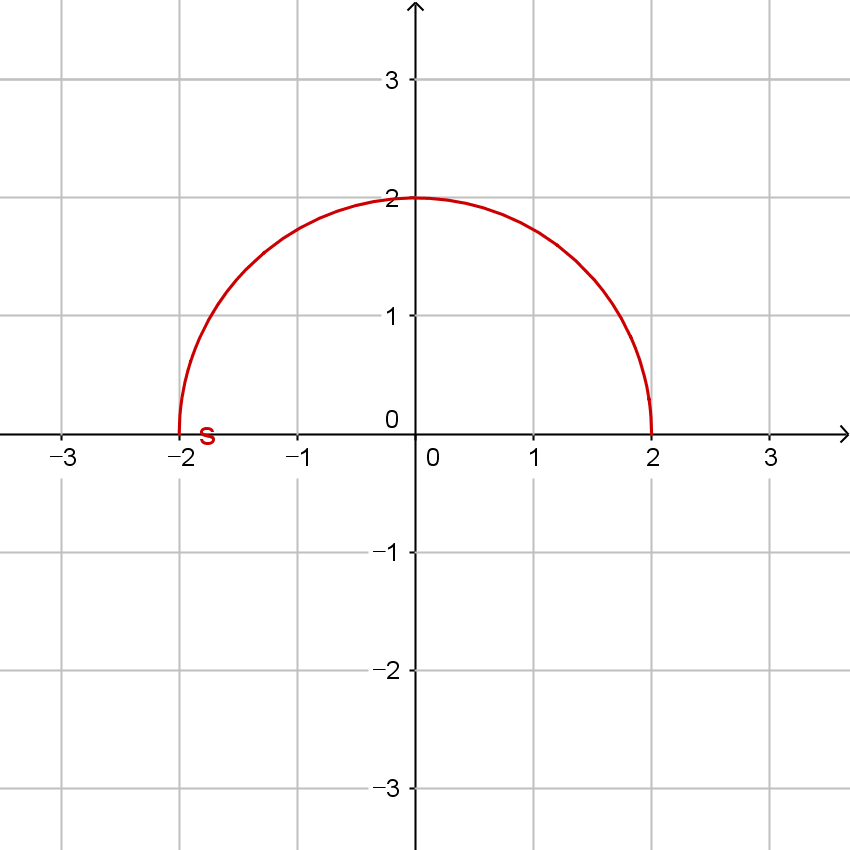
\includegraphics[width=0.45\textwidth]{pm3by3_hemisphere}
\par\noindent(3)\qquad\qquad\qquad\quad\:\:(4)
\end{center}
\begin{enumerate}[topsep=0pt]
\item
정의역=실수 전체 집합\\
치역=실수 전체 집합
\item
정의역=실수 전체 집합\\
치역=\(\{y\ba y\le2\}\)
\item
정의역=\(\{x\ba x\neq0\}\)\\
치역=\(\{y\ba y\neq0\}\)
\item
정의역=\(\{x\ba -2\le x\le2\}\)\\
치역=\(\{y\ba 0\le y\le2\}\)
\end{enumerate}

%
\an{28}
\(a=3\), \(b=-4\)
또는
\(a=-3\), \(b=8\)

%
\an{29}
\(4\), \(9\)
\end{minipage}
\end{document}